%%%%%%%%%%%%%%%%%%%%%%%%%%%%%%%%%%%%%%%%%%%%%%%%%%%%%%%%%%%%%%%%%%%%%%%%%%%%%%%
%%
%% Copyright © 2022 Tropic Square s.r.o. (https://tropicsquare.com/)
%%
%% This work is subject to the license terms of the LICENSE.txt file in the
%% root directory of this source tree.
%%
%% If a copy of the LICENSE file was not distributed with this work, you can
%% obtain one at (https://tropicsquare.com/license).
%%
%%%%%%%%%%%%%%%%%%%%%%%%%%%%%%%%%%%%%%%%%%%%%%%%%%%%%%%%%%%%%%%%%%%%%%%%%%%%%%%
%
% This is SPECT programmers manual
%
%%%%%%%%%%%%%%%%%%%%%%%%%%%%%%%%%%%%%%%%%%%%%%%%%%%%%%%%%%%%%%%%%%%%%%%%%%%%%%%

% Specify Tropic Square document class
\documentclass{tropic_design_spec}

\usepackage{listings}
\lstset{backgroundcolor=\color{lightgray}}

%%%%%%%%%%%%%%%%%%%%%%%%%%%%%%%%%%%%%%%%%%%%%%%%%%%%%%%%%%%%%%%%%%%%%%%%%%%%%%%
% Document properties and title page
%%%%%%%%%%%%%%%%%%%%%%%%%%%%%%%%%%%%%%%%%%%%%%%%%%%%%%%%%%%%%%%%%%%%%%%%%%%%%%%
\title{SPECT -- Programmer Guide}
\author{Vit Masek, Tropic Square}
\date{August 2023}

% Start of document
\begin{document}

% Parameters Needed by Design spec class (must be inside document)
% Set these parameters according to your project.
\def \projectname {SPECT}
\def \documentname {Programmer Guide ISAv0.2}
\def \versionnumber {0.6}

% Title page
\maketitle

\newcommand{\tspar}{\par\vspace{0.5cm}}
\newcommand{\tsspc}{\vspace{0.5cm}}
\newcommand{\tsblank}{\hspace*{0.5cm}}
\newcommand{\bi}[1]{\textbf{\textit{#1}}}

\newcommand{\tsnlind}{\newline\tsblank}

\newcommand{\tsif}{\textbf{\textit{if }}}
\newcommand{\tsthen}{\textbf{\textit{then: }}}
\newcommand{\tselse}{\newline\textbf{\textit{else: }}}

\def \G_RAR_DEPTH {5}


%%%%%%%%%%%%%%%%%%%%%%%%%%%%%%%%%%%%%%%%%%%%%%%%%%%%%%%%%%%%%%%%%%%%%%%%%%%%%%%
% Document revisions
%%%%%%%%%%%%%%%%%%%%%%%%%%%%%%%%%%%%%%%%%%%%%%%%%%%%%%%%%%%%%%%%%%%%%%%%%%%%%%%
\section*{Version history}

\begin{TropicRatioLongTable4Col}
    {0.1}            {0.2}                  {0.3}            {0.4}
    {Version Tag     & Date                 & Author          &    Description                    }
     0.1             & 12.10.2022           & Ondrej Ille     &    Initial version                      \Ttlb
     0.2             & 7.11.2022            & Ondrej Ille     &    Fix semantics of LSR instruction.    \Ttlb
     0.3             & 8.11.2022            & Ondrej Ille     &    Fix SCB semantics.                   \Ttlb
     0.4             & 14.11.2022           & Ondrej Ille     &    Fix semantics of ST instruction (op1 instead of op2).
                                                                   Add note about modular instruction operands. \Ttlb
     0.5             & 23.11.2022           & Ondrej Ille     &    Add description of SW toolchain.     \Ttlb
     0.6             & 9.8.2023             & Vit Masek       &    Move ISA descriptions to separate documents. \Ttlb
\end{TropicRatioLongTable4Col}

%%%%%%%%%%%%%%%%%%%%%%%%%%%%%%%%%%%%%%%%%%%%%%%%%%%%%%%%%%%%%%%%%%%%%%%%%%%%%%%
% External references
%%%%%%%%%%%%%%%%%%%%%%%%%%%%%%%%%%%%%%%%%%%%%%%%%%%%%%%%%%%%%%%%%%%%%%%%%%%%%%%

\newpage

\section*{Bibliography}

\begin{thebibliography}{9}

\bibitem{SHA512SPEC}
{FIPS 180-4}

\url{https://csrc.nist.gov/pubs/fips/180-4/upd1/final}

\bibitem{TROPIC01}
{TROPIC01 Repository}

\url{https://tropic-gitlab.corp.sldev.cz/internal/tropic01/tassic}

\bibitem{CRYPTOBLOCKS}
{ts-crypto-blocks}

\url{https://tropic-gitlab.corp.sldev.cz/internal/development-environment/ts-crypto-blocks}

\bibitem{SPECTFW}
{ts-spect-fw}

\url{https://tropic-gitlab.corp.sldev.cz/internal/sw-design/ts-spect-fw}

\bibitem{SCB}{
    Danger, Jean-Luc et al.
    “A synthesis of side-channel attacks on elliptic curve cryptography in smart-cards.”
    Journal of Cryptographic Engineering 3 (2013): 241 - 265.
}

\end{thebibliography}



%%%%%%%%%%%%%%%%%%%%%%%%%%%%%%%%%%%%%%%%%%%%%%%%%%%%%%%%%%%%%%%%%%%%%%%%%%%%%%%
% Table of contents
%%%%%%%%%%%%%%%%%%%%%%%%%%%%%%%%%%%%%%%%%%%%%%%%%%%%%%%%%%%%%%%%%%%%%%%%%%%%%%%
\pagebreak
\tableofcontents

%%%%%%%%%%%%%%%%%%%%%%%%%%%%%%%%%%%%%%%%%%%%%%%%%%%%%%%%%%%%%%%%%%%%%%%%%%%%%%%
%%%%%%%%%%%%%%%%%%%%%%%%%%%%%%%%%%%%%%%%%%%%%%%%%%%%%%%%%%%%%%%%%%%%%%%%%%%%%%%
% Document
%%%%%%%%%%%%%%%%%%%%%%%%%%%%%%%%%%%%%%%%%%%%%%%%%%%%%%%%%%%%%%%%%%%%%%%%%%%%%%%
%%%%%%%%%%%%%%%%%%%%%%%%%%%%%%%%%%%%%%%%%%%%%%%%%%%%%%%%%%%%%%%%%%%%%%%%%%%%%%%

%%%%%%%%%%%%%%%%%%%%%%%%%%%%%%%%%%%%%%%%%%%%%%%%%%%%%%%%%%%%%%%%%%%%%%%%%%%%%%%
% Glossary
%%%%%%%%%%%%%%%%%%%%%%%%%%%%%%%%%%%%%%%%%%%%%%%%%%%%%%%%%%%%%%%%%%%%%%%%%%%%%%%
\TsSection{Glossary}

\begin{itemize}
    \item{\textbf{CPU} - Central Processing Unit}
    \item{\textbf{ECC} - Elliptic Curve Cryptography}
    \item{\textbf{SPECT} - Secure Processor of Elliptic Curves for Tropic}
    \item{$P_{25519} = 2^{255} - 19$}
    \item{$P_{256} = 2^{256} - 2^{224} + 2^{192} + 2^{96} - 1$}
\end{itemize}

%%%%%%%%%%%%%%%%%%%%%%%%%%%%%%%%%%%%%%%%%%%%%%%%%%%%%%%%%%%%%%%%%%%%%%%%%%%%%%%
% Register field types
%%%%%%%%%%%%%%%%%%%%%%%%%%%%%%%%%%%%%%%%%%%%%%%%%%%%%%%%%%%%%%%%%%%%%%%%%%%%%%%
\TsSection{Register field types}

\TropicRegisterTypeList


%%%%%%%%%%%%%%%%%%%%%%%%%%%%%%%%%%%%%%%%%%%%%%%%%%%%%%%%%%%%%%%%%%%%%%%%%%%%%%%
% Introduction
%%%%%%%%%%%%%%%%%%%%%%%%%%%%%%%%%%%%%%%%%%%%%%%%%%%%%%%%%%%%%%%%%%%%%%%%%%%%%%%
\TsSection{Introduction}

This document provides a programmer's guide for SPECT. SPECT is a domain specific
processing unit targeted for calculations of Elliptic Curve Cryptography (ECC).
SPECT provides instructions for calculation with 256 bit numbers and modular
arithmetics. SPECT is useful to implement operations/algorithms such as:
\begin{itemize}
    \item{ECDSA -- Elliptic Curve Digital Signature Algorithm}
    \item{ECDH  -- Elliptic Curve Diffe-Hellman}
\end{itemize}

\begin{figure}[h!]
    \centering
    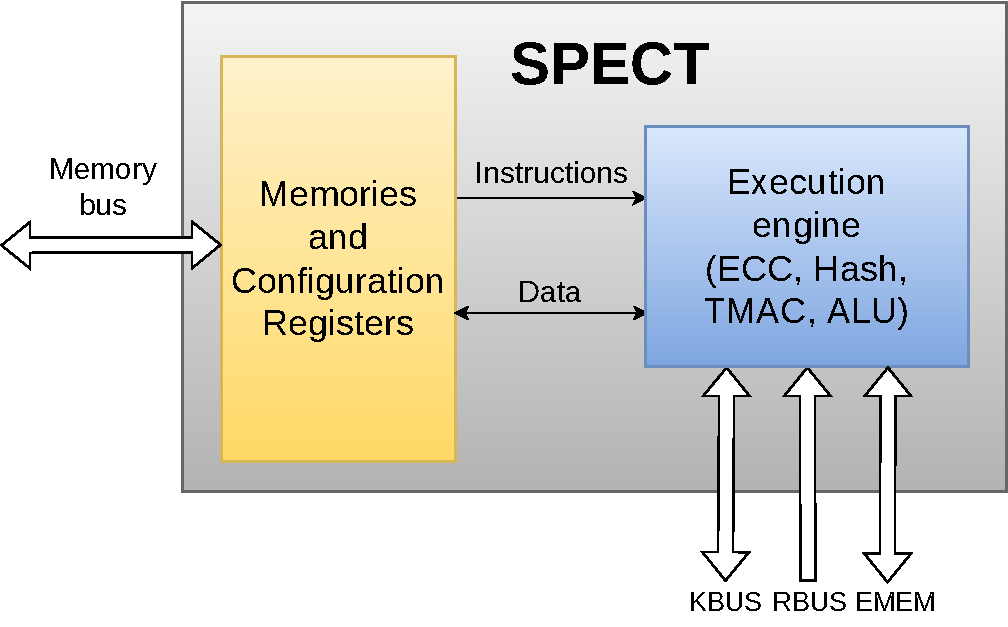
\includegraphics[width=\textwidth,height=\textheight,keepaspectratio]{%
        \detokenize{img/spect_pm_block_diagram.pdf}%
    }
    \caption{SPECT -- Block diagram}%
    \label{SPECTBK}%
\end{figure}

\TsSection{Programmer's model}

SPECT programmer's model consists of:
\begin{itemize}
    \item 32 x 256 bit general purpose registers (\textbf{R0} - \textbf{R31}).
    \item \textbf{PC} - Program counter.
    \item Zero (\textbf{Z}), Carry (\textbf{C}) and Error (\textbf{E}) flag.
    \item HW \textbf{RAR} (Return Address Register) stack for nested procedure calls.
    \item 2048 B read-write memory space in address range 0x0000 -- 0x07FC.
    \item 512 B write-only memory space in address range 0x1000 -- 0x11FC.
    \item 2048 B read-only memory space in address range 0x3000 -- 0x37FC.
    \item 144 B read-only memory space in address range 0x4000 -- 0x408C.\newline
        (from ISA v0.2)
    \item 50 B write-only memory space in address range 0x5000 -- 0x504C.\newline
        (from ISA v0.2)
\end{itemize}

\TropicNote{
    SPECTs address space is 32 bit word organized. Load and store
    instructions works with 256 bit values and it always uses 8 consecutive words
    in the memory. E.g. 0x0020 - 0x003C.
}

\begin{figure}[h!]
    \centering
    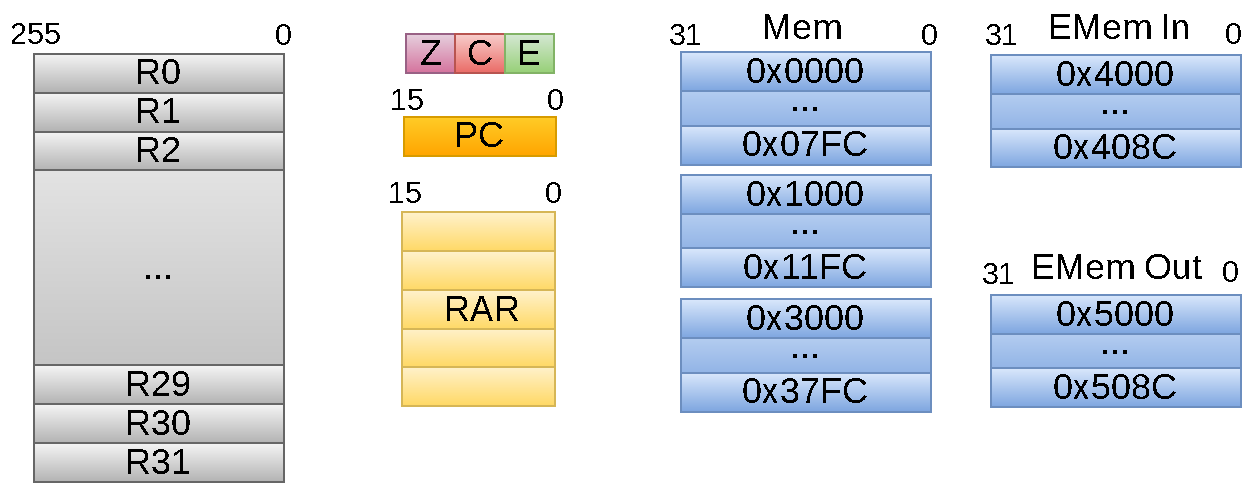
\includegraphics[width=.9\textwidth]{%
        \detokenize{img/spect_pm_gprs.pdf}%
    }
    \caption{SPECT -- Programmer model}%
    \label{SPECTBK}%
\end{figure}


\TsSubSection{Subroutine calls}

SPECT contains HW \textbf{RAR} stack, and it pushes return address from subroutine
to RAR stack each time when it executes CALL instruction. When SPECT executes
RET instruction, it pops value from RAR stack and updates \textbf{PC}. HW \textbf{RAR}
stack supports up to \G_RAR_DEPTH nested subroutine calls.

\TropicNote{
    Behavior of SPECT when number of nested subroutine calls is exceeded is undefined.
}

\TsSubSection{KBUS}

\textbf{From SPECT ISA v0.2}, SPECT HW implements special 32 bit BUS interface (KBUS) to store and load cryptographic keys.
Particular key within the system is identified by following parameters:
\begin{itemize}
    \item Type -- Type of the key (ECC, SHPUB, STPRIV etc.). It specifies the location
                  of tke key in the system.
    \item Slot -- Particular key slot of the specified type. One slot can contain multiple related keys
                  (E.g. scalar and prefix in case of EdDSA).
    \item Offset -- Offset within the slot. Specifies position of the particular key.
\end{itemize}

SPECT ISA provides three instruction for KBUS -- LDK, STK, KBO. LDK is used to load keys, STK to store keys
and KBO for further control of the KBUS. Because SPECT operates with 256 bit values, both LDK and STK execute 8
consecutive KBUS transactions incrementing the offset.

For purpose of this document, notation KBUS_READ[type,slot,offset] indicates result of 8 consecutive
KBUS read transactions (increasing offset). Data from the first transaction are considered as LSBs,
data from the last transaction are considered as MSBs.

Further, notation KBUS_WRITE[key,type,slot,offset] indicates 8 consecutive KBUS write transactions (increasing offset)
with wdata = key. In first transaction, wdata = key[31:0]. In the last transaction, wdata = key[255:223].
KBUS_OP[type,slot,op] indicates one KBUS transaction of specific OP (e.g. "program slot").

Fore more information about KBUS, see TROPIC01 Functional Specification, Section 19 \cite{TROPIC01}.

\TsSubSection{RBUS}

SPECT HW implements special 32 bit interface for requesting random numbers from the external systems RNG.
SPECT ISA provides possibility to fetch 256 bit random number with GRV instruction.

\TsSubSection{Modular arithmetics}

SPECT provides instructions for finite field arithmetic such as
addition, subtraction and multiplication with 256 bit operands stored in general purpose
registers. SPECT supports fast multiplication in Ed25519 and P-256 curves finite fields 
via dedicated instructions -- MUL25519 and MUL256. Modular arithmetics with generic modulus
specified by value in \textbf{R31} is supported by instructions ADDP, SUBP, MULP. SPECT
also supports modular reduction of 512 bit number with REDP instruction.

When programming with modular instructions, one needs to be careful about input
operands of such instructions. Following conditions must be met:
\begin{itemize}
    \item op2 < $P_{25519}$ and op3 < $P_{25519}$ for MUL25519 instruction.
    \item op2 < $P_{256}$ and op3 < $P_{256}$ for MUL256 instruction.
    \item op2 < R31 and op3 < R31 for ADDP, SUBP instructions.
    \item R31 != 0 and R31 != 1 for ADDP, SUBP, MULP, REDP instructions.
\end{itemize}
if these conditions are not met when invoking such a instruction, result
of the instruction calculation is undefined (value in op1).

\TropicNote{
    Performance of MULP when \textbf{R31} = $P_{25519}$ / $P_{256}$ is lower
    than performance of MUL25519 / MUL256.
}

\TsSubSection{SHA512}

SPECT HW supports SHA512 Hash calculation as specified in \cite{SHA512SPEC}. SPECT can
calculate SHA512 hash from arbitrarily long data stream. When SPECT executes HASH_IT
instruction, it resets context in its execution engine to initialization
vector as specified in \cite{SHA512SPEC}. Each execution of HASH instruction
processes 1024 bit block, and executes next round of SHA512 calculation.

\TropicNote{
    SPECT HW does not add any padding of input data. It is responsibility of the firmware or
    external system to add such padding.
}

\TsSubSection{TMAC}

\textbf{From SPECT ISA v0.2}, SPECT HW supports TMAC calculation as specified in TMAC documentation as part of ts-crypto-blocks repository \cite{CRYPTOBLOCKS}.
TMAC stands for Tropic Message Authentication Code. It is a custom MAC function inspired by KMAC function. It uses masked implementation
of KECCAK permutation with 400 bits internal state and rate of 18 bytes.

SPECT ISA provides four instructions for TMAC calculation.
\begin{itemize}
    \item TMAC_IT -- initialize underlying KECCAK core with 800 bits of mask and a guard.
    \item TMAC_IS -- initialize TMAC with initialization string as defined in TMAC specification.
    \item TMAC_UP -- updates internal state with another 18 bytes of data.
    \item TMAC_RD -- Squeeze 256 bits from the underlying KECCAK core as an output of the TMAC function.
\end{itemize}

\TsSubSection{Group Scalar Blinding}

SPECT HW supports scalar blinding by a random number as a side-channel counter-measure
with SCB instruction. It blinds the scalar $sc$ using group scalar randomization method
as defined in \cite{SCB} with 256 bit random number. The random number $rng$ shall be obtained in
advance by GRV instruction as described above. The group order $q$ shall be present in \textbf{R31}.

SCB performs this exact function: $$Blind(sc, rng, q) = q \times (rng | (2^{255} + 2^{223})) + sc$$

\TsSubSection{SPECT invocation}

SPECT firmware execution is invoked by external system that has access to its memory space via
memory bus as shown in following figure:

\begin{figure}[h!]
    \centering
    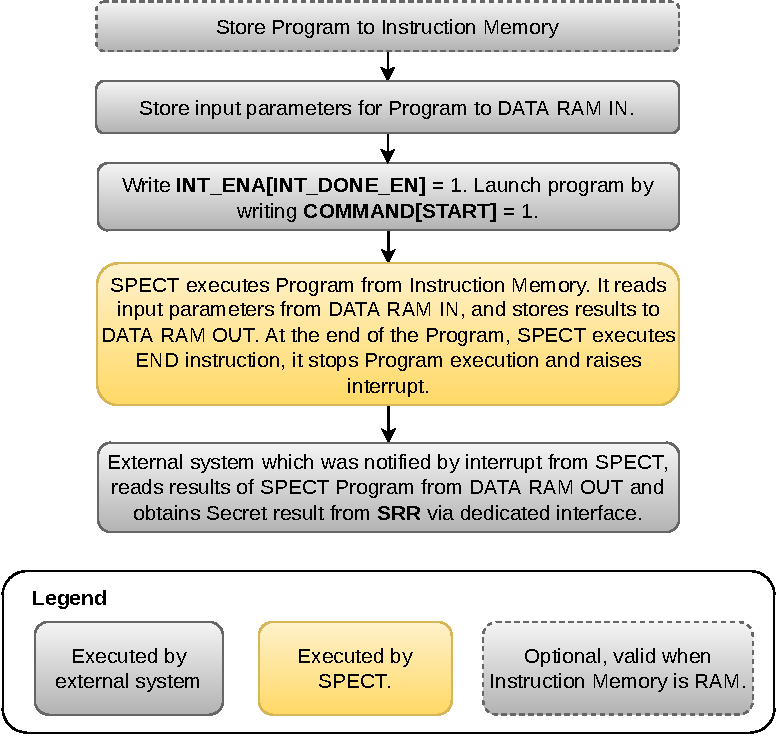
\includegraphics[width=.7\textwidth]{%
        \detokenize{img/spect_pm_invocation.pdf}%
    }
    \caption{SPECT -- Invocation}%
    \label{SPECTBK}%
\end{figure}

\TropicNote{
    Address of the first instruction executed by SPECT after
    \Register{COMMAND[START]} = 1 is written, is fixed and defined
    by a system that integrates SPECT.
}

\TsSubSection{Invalid instructions}

When SPECT attempts to execute invalid instruction, it aborts firmware execution
and sets \Register{STATUS[ERR]} = 1.

\TropicNote{
    Invalid instruction means invalid opcode or not matching parity bit in the instruction code. Unless
    a fault, usual cause of this is e.g. missing RET instruction in subroutine or END instruction at the
    end of the firmware execution.
}

\TsSubSection{Soft Reset}

SPECT can be reset by external system by writing \Register{COMMAND[SOFT_RESET]} = 1.
When SPECT is reset, it aborts any firmware execution and resets its internal state.

\TropicNote{
    Because GPRs are implemented as RAM, Soft Reset does not effect them in any way. GPRs can
    be cleared only by firmware.
}

\TsSubSection{Interrupts}

SPECT firmware execution can not be interrupted by an external event (other than
Soft Reset). SPECT itself can generate following interrupts for external system:
\begin{itemize}
    \item{Done -- Enabled when \Register{INT_ENA[INT_DONE_EN]} = 1.
                  Generated when SPECT firmware executes END instruction}
    \item{Error -- Enabled when \Register{INT_ENA[INT_DONE_EN]} = 1.
                   Generated when SPECT experience internal error (invalid instruction, bit-flip in SHA512 or TMAC core etc.)}
\end{itemize}


%%%%%%%%%%%%%%%%%%%%%%%%%%%%%%%%%%%%%%%%%%%%%%%%%%%%%%%%%%%%%%%%%%%%%
% 
% Autogenerated by TS Memory Map Generator
% Input: /projects/tropic01/work/vmasek/ts-spect/reg_map/spect_mem_map.yml
% Date: 09:38AM on May 11, 2023
%
%%%%%%%%%%%%%%%%%%%%%%%%%%%%%%%%%%%%%%%%%%%%%%%%%%%%%%%%%%%%%%%%%%%%%
%%%%%%%%%%%%%%%%%%%%%%%%%%%%%%%%%%%%%%%%%%%%%%%%%%%%%%%%%%%%%%%%%%%%%
% SPECT Memory Map
%%%%%%%%%%%%%%%%%%%%%%%%%%%%%%%%%%%%%%%%%%%%%%%%%%%%%%%%%%%%%%%%%%%%%
\pagebreak
\TsSection {SPECT Memory Map}

\textbf{Base Address:} 0x0000 0000
\newline
\textbf{End Address:} 0x0000 9FFF
\vspace{4mm}

\begin{TropicRatioTable3Col}
{0.6}                                         {0.3}                               {0.1}
{Memory region                                & Address offset range              & Size}

        \multirow {2} {*} {\hyperref[subsec:Data RAM IN] {Data RAM IN}} & 0x0000 0000 & \multirow {2} {*} {2 KB} \\
                                                    & 0x0000 07FF &    \Ttlb%
        
        \multirow {2} {*} {\hyperref[subsec:Data RAM OUT] {Data RAM OUT}} & 0x0000 1000 & \multirow {2} {*} {512 bytes} \\
                                                    & 0x0000 11FF &    \Ttlb%
        
        \multirow {2} {*} {\hyperref[subsec:Configuration registers] {Configuration registers}} & 0x0000 2000 & \multirow {2} {*} {16 bytes} \\
                                                    & 0x0000 200F &    \Ttlb%
        
        \multirow {2} {*} {\hyperref[subsec:Constants ROM] {Constants ROM}} & 0x0000 3000 & \multirow {2} {*} {2 KB} \\
                                                    & 0x0000 37FF &    \Ttlb%
        
        \multirow {2} {*} {\hyperref[subsec:External Memory In] {External Memory In}} & 0x0000 4000 & \multirow {2} {*} {64 bytes} \\
                                                    & 0x0000 403F &    \Ttlb%
        
        \multirow {2} {*} {\hyperref[subsec:External Memory Out] {External Memory Out}} & 0x0000 5000 & \multirow {2} {*} {80 bytes} \\
                                                    & 0x0000 504F &    \Ttlb%
        
        \multirow {2} {*} {\hyperref[subsec:Instruction Memory] {Instruction Memory}} & 0x0000 8000 & \multirow {2} {*} {8 KB} \\
                                                    & 0x0000 9FFF &    \Ttlb%
        
\end{TropicRatioTable3Col}

%%%%%%%%%%%%%%%%%%%%%%%%%%%%%%%%%%%%%%%%%%%%%%%%%%%%%%%%%%%%%%%%%%%%%
% Configuration registers
%%%%%%%%%%%%%%%%%%%%%%%%%%%%%%%%%%%%%%%%%%%%%%%%%%%%%%%%%%%%%%%%%%%%%
\pagebreak
\TsSubSection {Configuration registers}

\textbf{Base Address:} 0x0000 2000
\newline
\textbf{End Address:} 0x0000 200F
\vspace{4mm}
%   Ordt 230321.01 autogenerated file 
%   Input: /projects/tropic01/work/vmasek/ts-spect/reg_map/reg_map.rdl
%   Parms: /projects/tropic01/work/vmasek/ts-spect/doc/design_specification/temp_parms_files/reg_map.parms
%   Date: Thu May 11 09:38:24 CEST 2023
%

% Register Summary table
\begin{TropicRatioTable3Col}
{0.15} {0.65} {0.2}
{Address Offset & Register Name & Reset Value}
0x0 & \hyperlink{spect:BLOCK ID}{BLOCK_ID} & 0x000-0030\Ttlb%
0x4 & \hyperlink{spect:COMMAND}{COMMAND} & 0x00000000\Ttlb%
0x8 & \hyperlink{spect:STATUS}{STATUS} & 0x00000001\Ttlb%
0xc & \hyperlink{spect:INT ENA}{INT_ENA} & 0x00000000\Ttlb%
\end{TropicRatioTable3Col}

\pagebreak

\begin{landscape}

{\hypertarget{spect:BLOCK ID}{}}
\begin{TropicRegisterLandscapeTable}
  [Address:]%
  {BLOCK_ID}%
  {0x2000}%
  ID_CODE & RO & 0x30 & 15:0 & Identification code \Ttlb
  REV_CODE & RO & - & 19:16 & Revision code \Ttlb
\end{TropicRegisterLandscapeTable}


{\hypertarget{spect:COMMAND}{}}
\begin{TropicRegisterLandscapeTable}
  [Address:]%
  {COMMAND}%
  {0x2004}%
  START & WO W1S; & 0x0 & 0:0 & Starts SPECT FW operation \Ttlb
  SOFT_RESET & WO & 0x0 & 1:1 & Stops FW execution and resets SPECT \Ttlb
\end{TropicRegisterLandscapeTable}


{\hypertarget{spect:STATUS}{}}
\begin{TropicRegisterLandscapeTable}
  [Address:]%
  {STATUS}%
  {0x2008}%
  IDLE & RO & 0x1 & 0:0 & SPECT is in IDLE mode \Ttlb
  DONE & RW W1C & 0x0 & 1:1 & Active when SPECT successfully completes the calculation \Ttlb
  ERR & RW W1C & 0x0 & 2:2 & Active when SPECT ends the calculation with error \Ttlb
\end{TropicRegisterLandscapeTable}


{\hypertarget{spect:INT ENA}{}}
\begin{TropicRegisterLandscapeTable}
  [Address:]%
  {INT_ENA}%
  {0x200c}%
  INT_DONE_EN & RW & 0x0 & 0:0 & Enables DONE interrupt \Ttlb
  INT_ERR_EN & RW & 0x0 & 1:1 & Enables ERROR interrupt \Ttlb
\end{TropicRegisterLandscapeTable}


\end{landscape}


\TsSubSection{Data RAM IN}

Data RAM IN is a memory where external system stores parameters for SPECT firmware
before it starts its execution. SPECT firmware sees it as read-write memory.

\TsSubSection{Data RAM OUT}

Data RAM OUT is a memory where SPECT firmware stores results of its calculation,
and external system reads such results after SPECT firmware execution ends. SPECT
firmware sees it as write-only memory.

\TsSubSection{Instruction Memory}

Instruction memory contains the firmware executed by SPECT. External system preloads
the SPECT firmware to this memory in its boot up sequence.
SPECT firmware do not have access to this memory via load and store instructions. 

\TsSubSection{Constant ROM}

Constant ROM contains a ROM image with constants used by SPECT firmware (e.g. $P_{25519}$).
SPECT firmware sees it as read-only memory.

Content of such ROM is part of SPECT firmware repository. See \cite{SPECTFW}.

\TsSubSection{External Memory}

\textbf{From SPECT ISA v0.2}, SPECT HW implements special BUS interface (EMEM) to access different memory space within the external system.
There are two memories:
\begin{itemize}
    \item External Memory IN -- SPECT firmware sees it as read-only memory.
    \item External Memory OUT -- SPECT firmware sees it as write-only memory.
\end{itemize}

These memories are mapped in to SPECT memory space. Load and store instruction directs read / write transactions to
SPECTs memory subsystem or on to EMEM interface depending on the address in Addr field os the instruction.

%%%%%%%%%%%%%%%%%%%%%%%%%%%%%%%%%%%%%%%%%%%%%%%%%%%%%%%%%%%%%%%%%%%%%%%%%%%%%%%
% SPECT Assembler
%%%%%%%%%%%%%%%%%%%%%%%%%%%%%%%%%%%%%%%%%%%%%%%%%%%%%%%%%%%%%%%%%%%%%%%%%%%%%%%

\TsSection{SPECT Assembler}

SPECT assembler has support for following assembly language features:
\begin{itemize}
    \item{Function labels}
    \item{Constant definitions}
    \item{Include other assembly file}
    \item{Conditional compilation}
\end{itemize}

\TsSubSection{Tool requirements}

SPECT SW toolchain requires following tools:
\begin{itemize}
    \item CMAKE 3.18.2 or higher
\end{itemize}

\TsSubSection{Function labels}

SPECT compiler allows definition of function labels, and passing them
as NewPc of J instructions, e.g like so:

\begin{lstlisting}
_start:
    CALL my_func
    END

my_func:
    ADD r0, r1, r2
    RET
\end{lstlisting}

\TsSubSection{Constant definitions}

SPECT compiler allows definition of constants, and passing them as
Addr of M instructions or Immediate operand of I type instructions like so:

\begin{lstlisting}
threshold .eq 0x12

_start:
    ADDI r0, r0, threshold
\end{lstlisting}

\begin{lstlisting}
p25519_addr .eq 0x3020

_start:
    LD r31, p25519_addr
\end{lstlisting}

\TropicNote{
    Currently, SPECT compiler does not support expression parsing.
    It only supports simple decimal, hexadecimal or binary value
    when defining constants.
}

\TsSubSection{Include other assembly file}

Multiple .s assembly files can be connected together in SPECT source code
via "\texttt{.include}" directive, e.g. like so:

\begin{lstlisting}
_start:
    NOP

.include <other_s_file>
    END
\end{lstlisting}

\TsSubSection{Conditional compilation}

SPECT compiler supports conditional compilation using "\texttt{.ifdef}" directive.

\begin{lstlisting}
    .define MY_DEFINE
    .ifdef MY_DEFINE
        <some code>
    .else
        <some other code>
    .endif
\end{lstlisting}

By using "\texttt{-{}-isa-version=X}" switch of SPECT compiler or ISS, symbol\linebreak
"\texttt{SPECT_ISA_VERSION_<X>}" is defined automatically. The default value is the always newest ISA version.

%%%%%%%%%%%%%%%%%%%%%%%%%%%%%%%%%%%%%%%%%%%%%%%%%%%%%%%%%%%%%%%%%%%%%%%%%%%%%%%
% SW support
%%%%%%%%%%%%%%%%%%%%%%%%%%%%%%%%%%%%%%%%%%%%%%%%%%%%%%%%%%%%%%%%%%%%%%%%%%%%%%%
\TsSection{SW Toolchain}

SW toolchain intended for SW development and debugging SPECT firmware is available. The toolchain
has following applications available:

\begin{itemize}
    \item \texttt{spect_compiler} -- A compiler/assembler which creates .hex file from .s
                            assembly file.
    \item \texttt{spect_iss} -- Instruction set simulator with simple command line debugger.
                       It can simulate .s file as well as .hex file.
\end{itemize}

Options for each of the applications are described when using \texttt{-{}-help}
command line option. Options available inside interactive shell of
\texttt{spect_iss} are available with \texttt{-{}-help} command line option or \texttt{help}
command.

%%%%%%%%%%%%%%%%%%%%%%%%%%%%%%%%%%%%%%%%%%%%%%%%%%%%%%%%%%%%%%%%%%%%%%%%%%%%%%%
% Open issues
%%%%%%%%%%%%%%%%%%%%%%%%%%%%%%%%%%%%%%%%%%%%%%%%%%%%%%%%%%%%%%%%%%%%%%%%%%%%%%%
\TsSection{Open Issues}

\PrintOpenIssueSummary

\end{document}